\documentclass{acm_proc_article-sp}
\usepackage{graphicx}

\begin{document}

\title{The Future of Software Engineering with Consumer Virtual Reality}

\numberofauthors{3}
\author{
\alignauthor
Anthony Elliott\\
       \affaddr{North Carolina State University}\\
       \affaddr{Raleigh, North Carolina, USA}\\
       \email{anthony\_elliott@ncsu.edu}
\alignauthor
Brian Peiris\\
       \affaddr{Toronto, Ontario, Canada}\\
       \email{brian@fake.com}
\alignauthor
Chris Parnin\\
       \affaddr{North Carolina State University}\\
       \affaddr{Raleigh, North Carolina, USA}\\
       \email{chris.parnin@ncsu.edu}
}

\maketitle
\begin{abstract}
Virtual reality can provide huge benefits to software engineering.
Lorem ipsum dolor sit amet, consectetur adipiscing elit. Vestibulum semper a libero eu vulputate. Sed et mi ullamcorper felis sodales egestas vel et tortor. Vestibulum quis metus arcu. Pellentesque mattis magna nec turpis dignissim egestas. Praesent ut dignissim lorem. Mauris lacinia sem eget erat hendrerit, ac vestibulum dui tempus. Mauris quis tellus a leo porta vehicula et eu est. Maecenas ut quam eros. Praesent a molestie felis.
\end{abstract}

\section{Introduction}
Quality virtual reality (VR) is finally inexpensive enough for consumers, including software engineers, to invest in. No longer will we have to go to a physical room to be fully immersed in a virtual reality, within the next few years we will be able to simply reach over and put on our fully immersive VR sunglasses and headphones. Virtual reality is often applied only to the entertainment industry but we argue that it will greatly change software engineering as well. 

[Affordances of VR - lots of info, stereoscopic (true 3D), immersive]

Programmers have been tied to their monitors for too long. We stare at our three dimensional images on our two dimensional displays, unable to conceive of something greater. With VR we can truly be right next to the 3D graphics that we are creating. We can see the output of our system all around us, not just displayed on our second monitor.

Software has been limited by physical world. For instance, more and larger monitors can increase programmer productivity but budget and desk size constrain this issue.
Code review can be done in a physical room, but the room cannot be easily changed to show dynamic information. White-board walls can help this physical issue, but are still not as flexible as a completely virtual environment.

Virtual reality allows developers to interact with software in a more natural environment. This immersive environment allows users to process more information at once which in turn increases comprehension.

To immerse the user in a virtual environment we used a head-mounted display (Oculus Rift) and a Leap Motion Controller for gesture recognition. These devices are inexpensive (total is less than \$500) and could feasibly be used by a number of developers within five years.

Virtual reality has been around since Ivan Sutherland's Sword of Damocles in 1968 but the hardware is finally of high enough quality with a consumer price point. This will enable widespread adoption within the decade.

\begin{figure}[ht!]
\centering
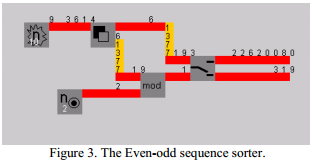
\includegraphics[width=70mm]{EvenOdd}
\caption{Possible setup with Rift \label{overflow}}
\end{figure}

[Describe each possible application in one sentence]

\begin{figure*}[ht]
\centering
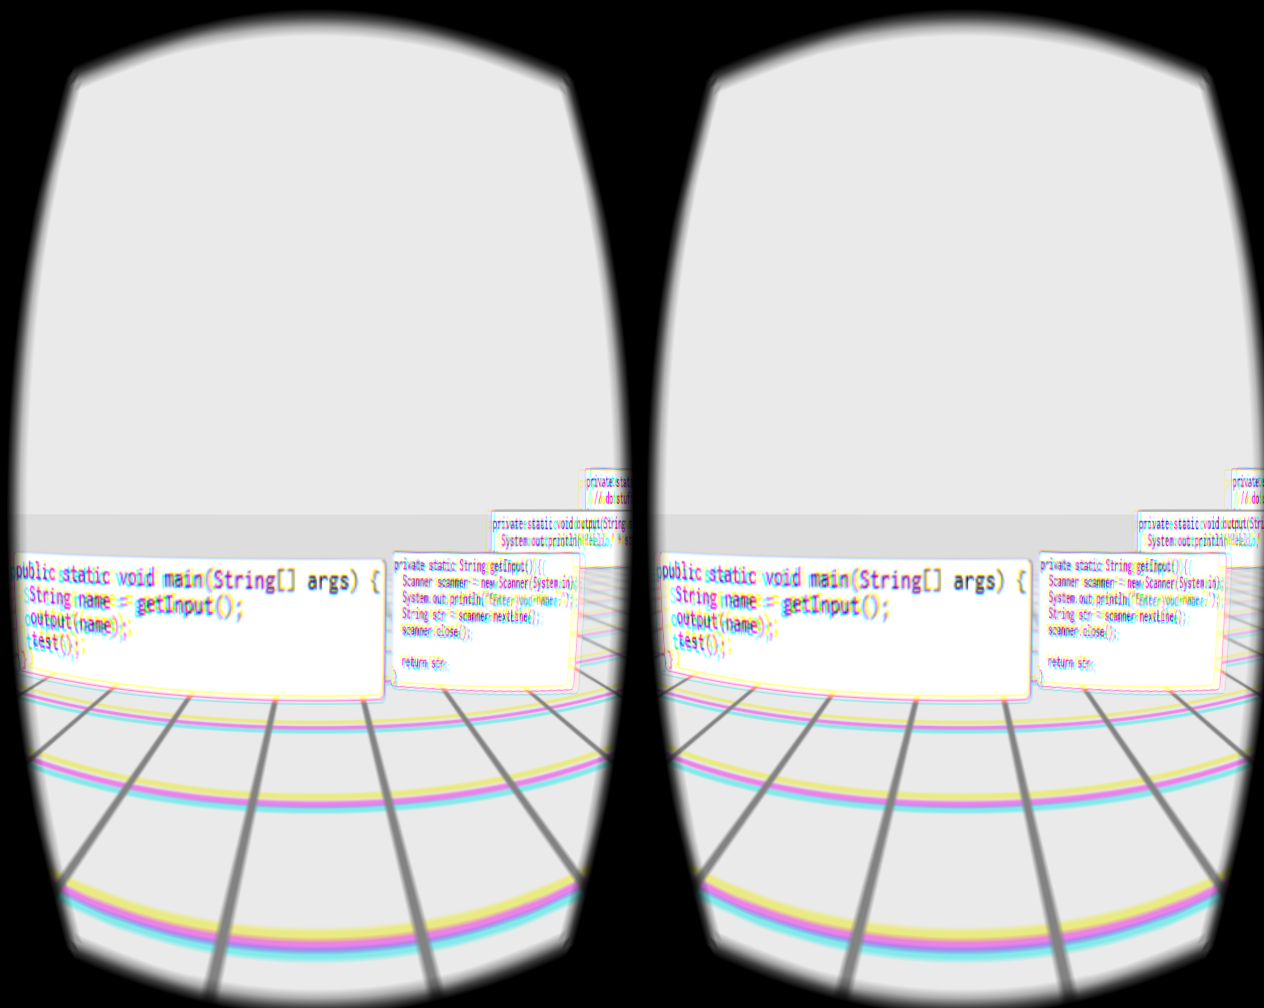
\includegraphics[width=\textwidth,height=5cm]{stack}
\caption{The active fragment is in the middle of the user's view. The user is currently looking at the implementations of the methods (shown to the right) called by the active fragment. The user is able to easily read 3 of these fragments at once.  \label{immersion}}
\end{figure*}

\section{Related Work}
Virtual environments called CAVEs have been around since the 1990's in which a person can be in a physical room with displays covering all surfaces.  Users often use head-mounted displays with head tracking to update the displays and may use hand-held devices to enable interaction with objects in the CAVE.

Andrew Bragdon has implemented a system called Code Bubbles that enables the user to pull out methods from a file. The user is then able to move and group the methods as desired.  Code Bubbles also can display the call graph for the selected method and allows the user to open called methods.

Code Canvas added semantic zoom to the Code Bubbles tool, allowing the user to gain a better understanding of how the current section of the system fits into the system as a whole.

Chris Parnin developed a tool called NosePrints which allows users to quickly see if a code smell is relevant~\cite{parnin:Noseprints}.

RoomAlive by Microsoft Research is similar to a CAVE but uses six Kinect sensors around the room to track the user.  This eliminates the need for wearable devices by the user but requires significant amounts of space.

\section{Applications}
% ties all application together
% take advantage of the affordances of VR
  % immersive env => lots of info at once
  % stereoscopic => true 3D; depth
Virtual environments can use the immersive property to display more information than on a computer monitor. We are still limited by the field of view of the human eye, so putting more information on the display is not novel, but what is novel is being able to distribute that information around the user in a meaningful way. This immersion is possible because the Rift uses stereoscopic rendering (creates a slightly different image for each eye) to enable depth sensing.

In this section we describe how VR could aid in code review, live coding, remote collaboration, and simulation. Our main contribution is not these specific ideas, but to show the possibilities of software engineering with VR.

\subsection{Code Review}
% Why does code review need another tool?
One of the primary motivations behind code reviews is to find defects in the code~\cite{bacchelli:ModernCodeReviewChallenges}. However, finding defects requires the reviewer to understand the code being modified~\cite{bacchelli:ModernCodeReviewChallenges}. It is especially hard if the reviewer has not touched this code in a long time and must reacquaint themselves with it.
% How manage the MSR citations above?

% What are the main benefits from using this tool?
  % affordances - immersive and more natural -- might be able to take out this paragraph if able to paint a good enough picture in their minds below
We propose a tool that takes advantage of the affordances of VR to help reviewers better understand the code being modified. This tool would be able to use the immersive environment to display more information to the user without them feeling overwhelmed. Additionally, the use of a device that can recognize hand gestures (such as the Leap Motion Controller) could allow reviewers to use interaction gestures that are more natural than a keyboard and mouse. 

  % display more info without being overwhelming
    % piles
      % able to get sense of size of pile
      % methods called by active fragment
    % git diff overview
    % complexity overview
    
 Imagine being able to see all of the code relevant to the current method but all on the same monitor. That sounds very cramped and overwhelming. What about being able to display each group of relevant code as a pile of fragments lying on the floor? The user could easily see that this active fragment is important because there are a lot of piles on the ground. Moreover, the user could get an idea of how much test code there is for the active fragment by simply gauging the size of the test code pile. [Describe different ideas for piles here]
 
 After assessing the piles of relevant information on the floor, the user can look to the left part of the sky and see an overview of the changes made in this review. [talk more about git diff here]
 The user could also easily take in other useful visualizations such as an overview of the complexity of the different parts of the system and where the current fragment fits into the big picture.
    
  % still able to see details
    % active fragment
    % detailed view (stack/circle) of fragments
    
 If the user wants to look at the implementation of the methods called by the active fragment, they could simply reach out in the direction of the pile, grab it with their hand and pull their hand up. The fragments in the pile would follow the hand up and form a circle to the right of the active fragment. The user would then be able to read the details of the called methods at the forefront of the circle. The user could make a three-fingered swipe to the left to rotate the circle and bring the next three fragments to the forefront.  The user finds an especially large method, grabs it using a pinch motion on the top and bottom and moves it on top of the active fragment. The piles change to include code relevant to the new fragment.  The user realizes that this new fragment is only used once since that 'pile' only had one  fragment in it. She moves her arm as if she were clearing off her desk and returns to the fragment she initially had active.
    
  % interaction
    % grab pile
    % pull hand up to pull pile into detailed view
    % push hand down to push detailed view back into pile on floor
    % swipe with fingers to cycle through detailed view
      % three finger swipe could cycle three fragments
    % change active fragment somehow
    

% What makes a VR code review tool better than a 3D tool displayed on a monitor?
  % immersive (try to make this obvious from the above section)

[Conclude and repeat how this tool could help developers rather than just looking cool]

\subsection{Livecoding}
RiftSketch

\begin{figure}[ht!]
\centering
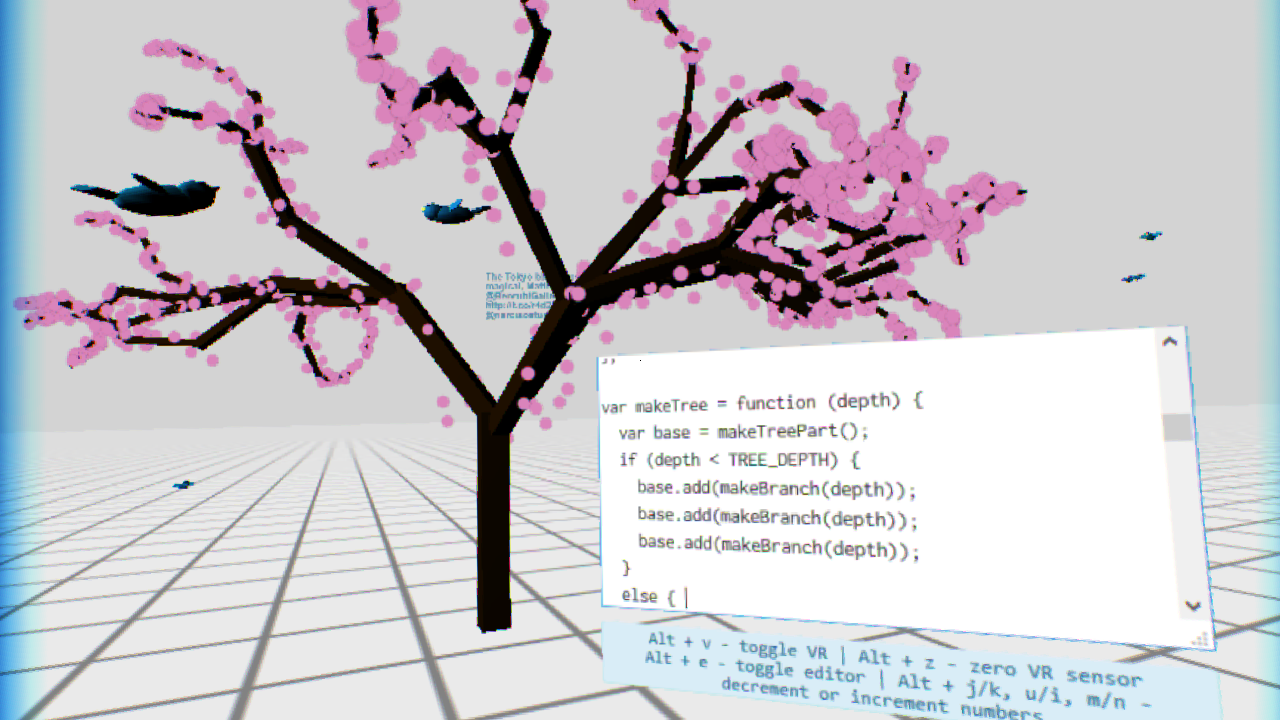
\includegraphics[width=80mm]{figures/riftsketch/closer}
\caption{RiftSketch screenshot \label{riftsketch}}
\end{figure}

RiftSketch is a live coding environment built for VR. It allows a user to describe a 3D scene using geometries, materials, textures, lights, meshes and other primitives provided by the Three.js library, which is a convenient wrapper for the WebGL APIs available in modern browsers. RiftSketch presents a user with a simple text editor, floating in front of them in an otherwise empty VR world. As the user types code into the editor, the world around them updates instantly to display the 3D scene dictated by their code. RiftSketch also allows the user to animate their scene via a callback function which is executed on every frame. The user can manipulate the state of the 3D scene in this looped block of code in order to add behaviour to the objects in their scene.

Furthermore, RiftSketch provides the user with shortcuts and input methods to quickly edit numbers in the code that they write. Keyboard shortcuts allow the user to increment or decrement numbers in the code by increments of 0.1, 10 or 100. Integration with the Leap Motion Controller provides users with the ability to manipulate numbers using natural input: the user places the editor's cursor over a number and then can move their hand up and down above the Leap Motion controller in order to increase or decrease the number. Numbers in the code could represent anything, from the X,Y or Z components of a position or rotation vector, the red, green or blue components of an object's material or a component in the calculation of an object's animated speed.

Although the current implementation of RiftSketch is little more than a creative toy, the experience of using it shows the potential of practical applications. Largely inspired by Bret Victor's seminal lecture, "Inventing on Principle" [1][2], RiftSketch demonstrates the potency of giving a creator, or programmer, a direct and immediate connection to their creation. This tight feedback loop allows the programmer to better understand the effect of every part of the code that they write and to quickly experiment with various solutions, algorithms and calculations. RiftSketch is also very effective as a learning tool since users can see their mistakes immediately and correct themselves without an intermediate compile step that might otherwise act as a roadblock.  These benefits are especially evident in RiftSketch when the code describes a VR scene. Watching the entire virtual world change around you as you type can be an extremely powerful and engaging experience.

In practical applications, one could extend the concept of live coding and tight feedback loops in order to create customized programming environments. VR programming environments could allow the user to take advantage of the malleability and expanse of virtual worlds. For example, a user could live code a widget that indicates some statistic of the code they are currently editing, such as the cyclomatic complexity, test coverage or test result. The widget would update itself as the user typed, not unlike existing code feedback tools such as NCrunch[3], and they could position the widget in their virtual periphery.

VR worlds are also well-suited to applications with physical analogs that can be simulated in 3D. For example, if a programmer was working on avionics software in a live coding environment, the VR world could include a simulation of a plane with moving control surfaces, propellers or a visualization of the aircraft's fuel injection system. The live coding environment would then give the programmer immediate visual feedback about the control flow and logic that they were programming. The programmer could scale the virtual plane to a manageable size to give her an overview of its behaviour, scale it to normal size and walk around the plane to inspect a particular control surface or scale it to larger than life-size, transport herself into the guts of the plane to watch a particular fuel valve respond to the state of the program.

[1] - "Inventing on Principle" Vimeo. Bret Victor, 19 Jan. 2012. Web. 11 Nov. 2014. <http://vimeo.com/36579366>.
[2] - "Transcript of Bret Victor's 'Inventing on Principle' talk" GitHub. Edward Z. Yang, 22 Aug. 2013. Web. 11 Nov. 2014. <https://github.com/ezyang/cusec2012-victor/blob/master/transcript.md>.
[3] - "NCrunch automated concurrent testing tool" NCrunch. NCrunch, 18 Sept. 2014. Web. 11 Nov. 2014. <http://www.ncrunch.net/>.

\subsection{Remote Collaboration}
% Imagining room inside HiFi with multiple avatars
% each developer could have an avatar
% able to get facial expressions
% able to get body language (although somewhat expensive right now, these prices will come down)

% code review
% pair programming
  % pair 'live coding'
  % pair designing
% exploring data visualization together

Lorem ipsum dolor sit amet, consectetur adipiscing elit. Vestibulum semper a libero eu vulputate. Sed et mi ullamcorper felis sodales egestas vel et tortor. Vestibulum quis metus arcu. Pellentesque mattis magna nec turpis dignissim egestas. Praesent ut dignissim lorem. Mauris lacinia sem eget erat hendrerit, ac vestibulum dui tempus. Mauris quis tellus a leo porta vehicula et eu est. Maecenas ut quam eros. Praesent a molestie felis. Suspendisse imperdiet ligula ac ante cursus, vitae dignissim elit rhoncus. Suspendisse sapien massa, rutrum non luctus in, accumsan eget velit. Nam mollis, ligula eget porta gravida, nibh mi euismod turpis, eget fermentum elit velit quis eros.

Duis aliquam tempor odio, ac cursus justo condimentum ac. Nulla ligula dui, lobortis sed magna ut, feugiat dictum eros. Maecenas cursus tincidunt dui vitae mattis. Cras dictum id libero non scelerisque. Nunc fermentum est turpis. Quisque porttitor congue arcu. Nam auctor iaculis aliquam. Etiam tempor pellentesque dui, at ullamcorper leo bibendum et. Praesent dictum erat nec dignissim posuere. Nam eu aliquet purus, viverra feugiat lectus. Maecenas posuere diam et lacus feugiat, quis consectetur ante venenatis. Praesent lobortis lacus non vestibulum rhoncus.

Pellentesque rutrum libero vitae massa consequat molestie. Nullam rutrum convallis ligula sed feugiat. Sed non imperdiet nisl. Ut at vulputate diam. Etiam ullamcorper efficitur libero, eu fringilla dui semper quis. Donec sapien elit, rhoncus vitae ullamcorper vitae, malesuada et diam. Pellentesque habitant morbi tristique senectus et netus et malesuada fames ac turpis egestas. Donec semper, dolor non tempus cursus, diam tortor iaculis nulla, at semper nulla elit sed sapien. Proin egestas, sem laoreet posuere vulputate, neque nisi euismod mi, id efficitur leo diam eget turpis. Donec accumsan mollis ex, at maximus justo posuere non. Sed venenatis, neque vitae vehicula porttitor, urna eros consectetur tortor, non rutrum felis nisl sit amet nisl. Proin vitae tempor arcu, ac pharetra mauris. Nam eros ipsum, consequat id ex et, gravida maximus massa.

\subsection{Simulation}

Lorem ipsum dolor sit amet, consectetur adipiscing elit. Vestibulum semper a libero eu vulputate. Sed et mi ullamcorper felis sodales egestas vel et tortor. Vestibulum quis metus arcu. Pellentesque mattis magna nec turpis dignissim egestas. Praesent ut dignissim lorem. Mauris lacinia sem eget erat hendrerit, ac vestibulum dui tempus. Mauris quis tellus a leo porta vehicula et eu est. Maecenas ut quam eros. Praesent a molestie felis. Suspendisse imperdiet ligula ac ante cursus, vitae dignissim elit rhoncus. Suspendisse sapien massa, rutrum non luctus in, accumsan eget velit. Nam mollis, ligula eget porta gravida, nibh mi euismod turpis, eget fermentum elit velit quis eros.

Duis aliquam tempor odio, ac cursus justo condimentum ac. Nulla ligula dui, lobortis sed magna ut, feugiat dictum eros. Maecenas cursus tincidunt dui vitae mattis. Cras dictum id libero non scelerisque. Nunc fermentum est turpis. Quisque porttitor congue arcu. Nam auctor iaculis aliquam. Etiam tempor pellentesque dui, at ullamcorper leo bibendum et. Praesent dictum erat nec dignissim posuere. Nam eu aliquet purus, viverra feugiat lectus. Maecenas posuere diam et lacus feugiat, quis consectetur ante venenatis. Praesent lobortis lacus non vestibulum rhoncus.

Pellentesque rutrum libero vitae massa consequat molestie. Nullam rutrum convallis ligula sed feugiat. Sed non imperdiet nisl. Ut at vulputate diam. Etiam ullamcorper efficitur libero, eu fringilla dui semper quis. Donec sapien elit, rhoncus vitae ullamcorper vitae, malesuada et diam. Pellentesque habitant morbi tristique senectus et netus et malesuada fames ac turpis egestas. 

\section{Open Research Questions}
% VR vs AR in the future, which is better?
  % code snippets while wearing Google Glass could appear on peripherals
We have presented virtual environments that completely immerse the user. Other devices such as Google Glass, aim to help the user complete tasks in the physical world by adding information overlays (augmented reality). Augmented reality seeks to help the user in the physical world while virtual reality seeks to completely replace physical reality. 
Is it more useful to immerse the user in a completely virtual, dynamic environment, or to enhance the physical world of developers?
  
% Manipulating environment
% Utilize the 'experience'?
  % Gamification of code review
% Where is the limit for too much info displayed at once?
% One main focal point (e.g. active fragment) or better to switch position to see other important things?
  % With Immersion, the user is focused on the active fragment and I will use the peripherals for some extra info that isn't quite so important. This requires the user to rotate their head.
  % But if I had a room then it would be much easier to have the user completely change their position (the Rift makes this uncomfortable with the wires)
  % So if I had better equipment, would it be better to make one 'wall' primary and all others secondary or to allow all of them to become primary?
% Does using a VR code review tool actually increase comprehension? Does it allow users to find bugs and provide alternative solutions?
% What gestures are most natural in VR?
% What use the z-axis for?
% Use VR for specific activities?
% Will a developer buy a Rift just for the tools?

Lorem ipsum dolor sit amet, consectetur adipiscing elit. Vestibulum semper a libero eu vulputate. Sed et mi ullamcorper felis sodales egestas vel et tortor. Vestibulum quis metus arcu. Pellentesque mattis magna nec turpis dignissim egestas. Praesent ut dignissim lorem. Mauris lacinia sem eget erat hendrerit, ac vestibulum dui tempus. Mauris quis tellus a leo porta vehicula et eu est. Maecenas ut quam eros. Praesent a molestie felis. Suspendisse imperdiet ligula ac ante cursus, vitae dignissim elit rhoncus. Suspendisse sapien massa, rutrum non luctus in, accumsan eget velit. Nam mollis, ligula eget porta gravida, nibh mi euismod turpis, eget fermentum elit velit quis eros.

Duis aliquam tempor odio, ac cursus justo condimentum ac. Nulla ligula dui, lobortis sed magna ut, feugiat dictum eros. Maecenas cursus tincidunt dui vitae mattis. Cras dictum id libero non scelerisque. Nunc fermentum est turpis. Quisque porttitor congue arcu. Nam auctor iaculis aliquam. Etiam tempor pellentesque dui, at ullamcorper leo bibendum et. Praesent dictum erat nec dignissim posuere. Nam eu aliquet purus, viverra feugiat lectus. Maecenas posuere diam et lacus feugiat, quis consectetur ante venenatis. Praesent lobortis lacus non vestibulum rhoncus.

Pellentesque rutrum libero vitae massa consequat molestie. Nullam rutrum convallis ligula sed feugiat. Sed non imperdiet nisl. Ut at vulputate diam. Etiam ullamcorper efficitur libero, eu fringilla dui semper quis. Donec sapien elit, rhoncus vitae ullamcorper vitae, malesuada et diam. Pellentesque habitant morbi tristique senectus et netus et malesuada fames ac turpis egestas. Donec semper, dolor non tempus cursus, diam tortor iaculis nulla, at semper nulla elit sed sapien. Proin egestas, sem laoreet posuere vulputate, neque nisi euismod mi, id efficitur leo diam eget turpis. Donec accumsan mollis ex, at maximus justo posuere non. Sed venenatis, neque vitae vehicula porttitor, urna eros consectetur tortor, non rutrum felis nisl sit amet nisl. Proin vitae tempor arcu, ac pharetra mauris. Nam eros ipsum, consequat id ex et, gravida maximus massa.

\section{Conclusions}

Lorem ipsum dolor sit amet, consectetur adipiscing elit. Vestibulum semper a libero eu vulputate. Sed et mi ullamcorper felis sodales egestas vel et tortor. Vestibulum quis metus arcu. Pellentesque mattis magna nec turpis dignissim egestas. Praesent ut dignissim lorem. Mauris lacinia sem eget erat hendrerit, ac vestibulum dui tempus. Mauris quis tellus a leo porta vehicula et eu est. Maecenas ut quam eros. Praesent a molestie felis. Suspendisse imperdiet ligula ac ante cursus, vitae dignissim elit rhoncus. Suspendisse sapien massa, rutrum non luctus in, accumsan eget velit. Nam mollis, ligula eget porta gravida, nibh mi euismod turpis, eget fermentum elit velit quis eros.


\bibliographystyle{abbrv}
\bibliography{nier2015_Immersion}
\end{document}
